\documentclass[../documentation.tex]{subfiles}
 
\begin{document}
\section{Robotkar mozgásának definiálása és programozása}
\subsection{Biztonsági beállítások}
Ahhoz hogy a robot működése során ne jelentsen veszélyt a munkaterében lévő emberekre és vagyontárgyakra, különböző biztonsági eszközök beszerelésére, illetve akitválására van szükség. A robotszoftverben implementált biztonsági funkciók között vannak módosítható és permanens elemek. Ezeket foglalja össze felsorolás jelleggel \aref{sec:safetyfunctions} fejezet. A továbbiakban csak a projekt során is aktív elemek kerülnek tárgyalásra.

\subsubsection{Vészleállító eszköz}
Az ipari robot esetében a vészleállító eszköz (\angol{EMERGENCY STOP	 device}) a smartPAD-en található vészleállító (\ref{fig:smartpad} ábra). Ezt a kapcsolót kockázatos szituációban vagy vészhelyzetben kötelező benyomni.

Ha az operátor benyomta a vészleállító gombot, akkor a robotkar \angol{Safety stop 1 (path-maintaining)} (leírás \aref{tab:terms} táblázatban) megállást hajt végre. Az EMERGENCY STOP eszközt el kell csavarni ahhoz, hogy a műveletek folytatódhassanak.

\subsubsection{Engedélyező eszköz}
A robotkar esetében az engedélyező eszközök (\angol{enabling devices}) a smartPAD-re szerelt engedélyező kapcsolók. 3 ilyen kapcsoló található a smartPAD-en (\ref{fig:smartpad} ábra). Ezek mindegyikének 3 állása van:
\begin{itemize}
	\item Nem behúzott
	\item Középső pozíció
	\item Teljesen behúzott (pánik pozíció)
\end{itemize}

A teszt módokban és CRR esetén (\ref{tab:terms}) a robotkar csak akkor mozgatható, ha legalább 1 engedélyező kapcsoló középső állásban van.
\begin{itemize}
	\item Az engedélyező kapcsoló elengedése \angol{Safety stop 1 (path-maintaining)} megállást fog okozni.
	\item A kapcsoló teljes behúzása is ugyanilyen megálláshoz vezet.
	\item 2 engedélyező kapcsolót a középső pozícióban tartani lehetséges néhány másodpercig. Ez lehetőséget ad arra, hogy az operátor fogást váltson. Ha 2 engedélyező kapcsoló párhuzamosan középső pozícióban van tartva 15 másodpercnél tovább, az szintén \angol{Safety stop 1 (path-maintaining)} megállást fog okozni.
\end{itemize}

Ha az engedélyező kapcsoló a középső állásban ragad, akkor a következő lehetőségek állnak rendelkezésre:
\begin{itemize}
	\item a kapcsoló teljes behúzása,
	\item az EMERGENCY STOP eszköz benyomása,
	\item illetve a Start gomb elengedése
\end{itemize}

\begin{figure}[h]
    \centering
    \begin{subfigure}[t]{0.5\textwidth}
        \centering
        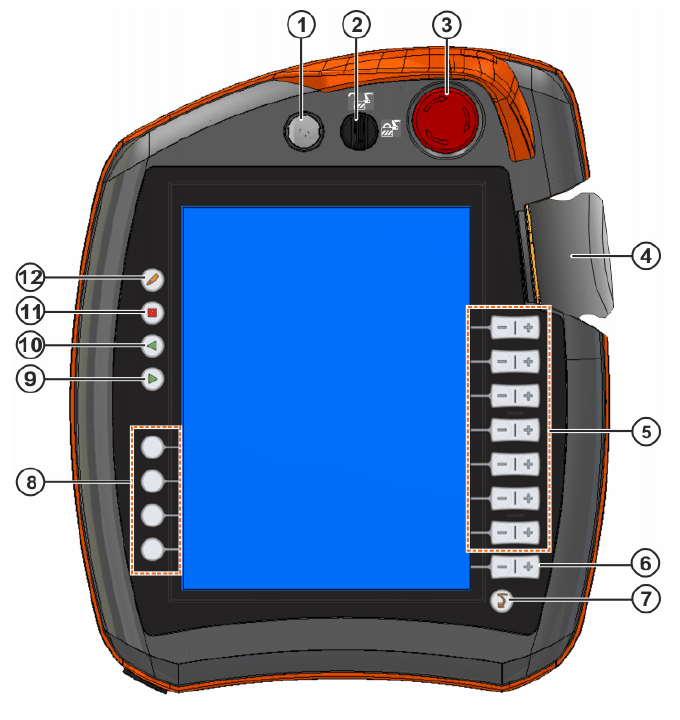
\includegraphics[scale=0.4]{smartpad-front}
        \caption{smartPAD előlnézetből\\ 2: kulcsos kapcsoló\\ 3: EMERGENCY STOP eszköz \\ 9: Start gomb}
    \end{subfigure}%
    ~ 
    \begin{subfigure}[t]{0.5\textwidth}
        \centering
        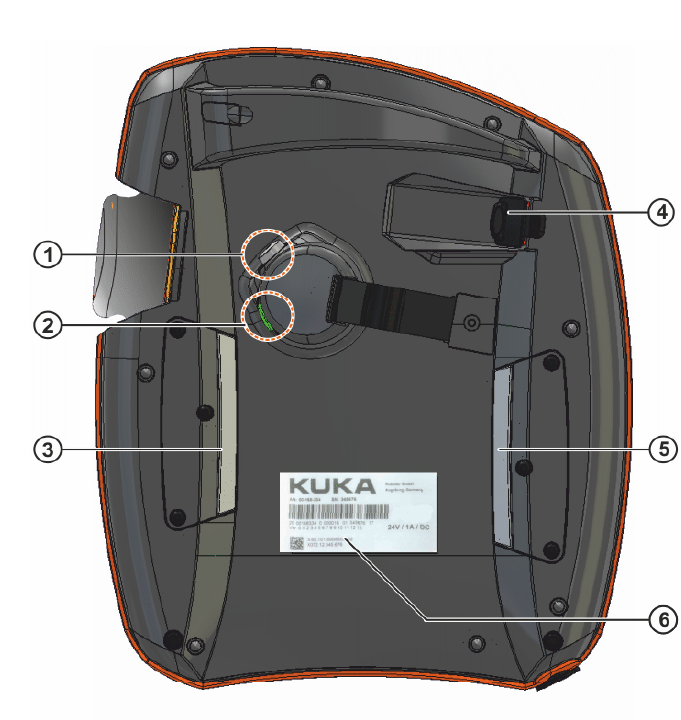
\includegraphics[scale=0.4]{smartpad-rear}
        \caption{smartPAD hátulnézetből\\ 1, 3, 5: enegedélyező kapcsoló\\ 2: Start gomb}
    \end{subfigure}
    \caption{KUKA smartPad\cite{sunrisemanual}}
    \label{fig:smartpad}
\end{figure}

\subsubsection{Operációs mód rögzítése}
Ahhoz hogy a robot mozgása közben ne lehessen operációs módot váltani (pl.: T1 módból T2-be), a smartPAD-en található egy kulcsos kapcsoló (\ref{fig:smartpad} ábra). Ennek elfordítására a robot megáll, ekkor lehet tetszőleges operációs módot választani. Ezeket \aref{tab:terms} táblázat részletesen tartalmazza.

\subsubsection{Megállást előidéző események}
A sakkprojekt során az alábbi események megállást idézhetnek elő a program futása során (a csillagozott elemek permanensen a robotszoftverbe vannak programozva, ezeket módosítani nem lehet):
\begin{itemize}
	\item operációs mód váltás történt mozgás közben*,
	\item az engedélyező kapcsolót elengedték*,
	\item az engedélyező kapcsolót teljesen behúzták*,
	\item a smartPAD-en található \angol{EMERGENCY STOP} eszközt benyomták*,
	\item a tengelyekre előírt maximális többletnyomatékot valamelyik tengelyen meghaladja a terhelés.
\end{itemize}

\subsection{Mozgástípusok elméletben}
Ez a fejezet bemutatja a mozgások programozásának elméleti szabályait. A szakdolgozat során programozott elemeket \aref{sec:motionprogramming} fejezet tárgyalja.

\subsubsection{Mozgástípusok áttekintése}
Több egymás utáni mozgás végrehajtása során a mozgás kezdőpontja mindig az előző végpontja.
A következő mozgástípusokat lehet beprogramozni különálló mozdulatokként:
\begin{itemize}
	\item Point-to-point (PTP, Ponttól pontig)
	\item Lineáris mozgás (LIN)
	\item Körkörös mozgás (\angol{Circural motion}, CIRC)
	\item Manuális vezetés kézi vezető eszközzel
\end{itemize}

A következő mozgástípusokat lehet beprogramozni a CP (``\angol{Continuous Path}'' - ``folytonos út'') spline\footnote{A mozgatott pont spline mentén halad a térben} blokk\cite{sunrisemanual} részeként:
\begin{itemize}
	\item Lineáris mozgás (LIN)
	\item Körkörös mozgás (\angol{Circural motion}, CIRC)
	\item Polinomiális mozgás (SPL)
\end{itemize}

JP (``\angol{Joint Path}'' - ``tengely út'') spline\footnote{Mivel a robotkar 7 tengellyel rendelkezik, a mozgása közben a tengelyek állása nem egyértelmű. JP sline blokk kivitelezésénél a tengelyek szögsebessége folytonos, így egy kedvezőbb dinamikájú mozdulatsort visz véghez.} blokk\cite{sunrisemanual} programozásakor PTP elemeket lehet használni.

A LIN, CIRC, SPL, CP spline blokk mozdulatok CP (``\angol{Continuous Path}'') típusúak, míg a PTP és a JP spline blokk JP (``\angol{Joint Path}'' - ``tengely út'') típusúak.

\subsubsection{PTP mozgástípus}
A robot a TCP-t a leggyorsann úton vezeti el a végponthoz. A leggyorsabb út általában nem egyezik meg a térbeli legrövidebbel, tehát nem egy egyenes (\ref{fig:ptpmotion}). A görbe útvonalak lekövetése gyorsabb az egyenesnél, mivel a robot tengelyei forogva és szimultán mozognak.

PTP a gyors pozícionáló mozgás. A mozgás pontos útvonala nem előre megjósolható, de többszöri futtatásra is ugyanazt az útvonalat követi le, feltéve ha az általános feltételek nem változtak.

\begin{figure}[h]
    \centering
    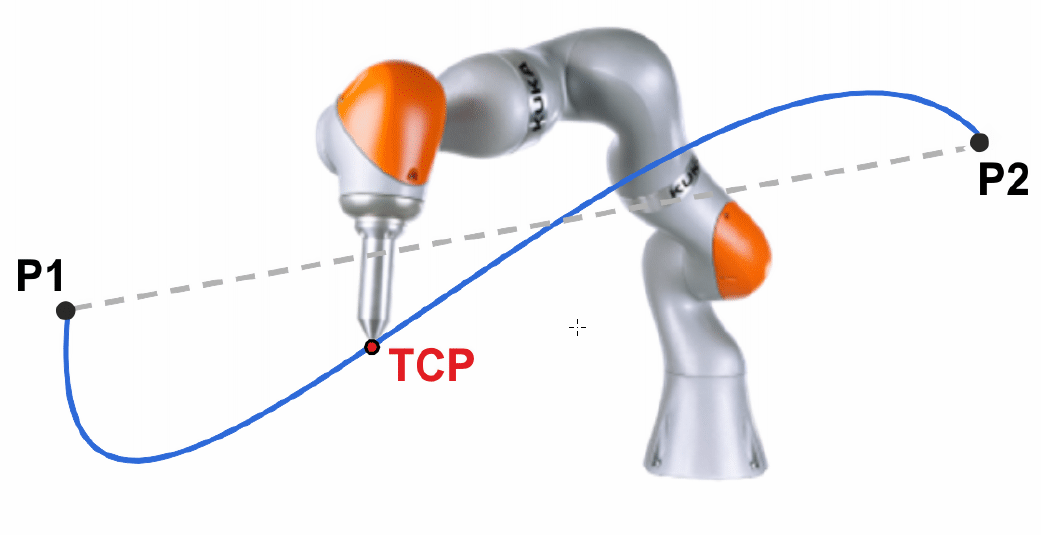
\includegraphics[scale=0.4]{ptpmotion}
    \caption{PTP mozgás\cite{sunrisemanual}}
    \label{fig:ptpmotion}
\end{figure}

\subsubsection{LIN mozgástípus}
A robot a TCP-t egy térbeli egyenes mentén mozgatja a végponthoz. A LIN mozgás során a végpozíció konfigurációját a program nem veszi figyelembe.

\begin{figure}[h]
    \centering
    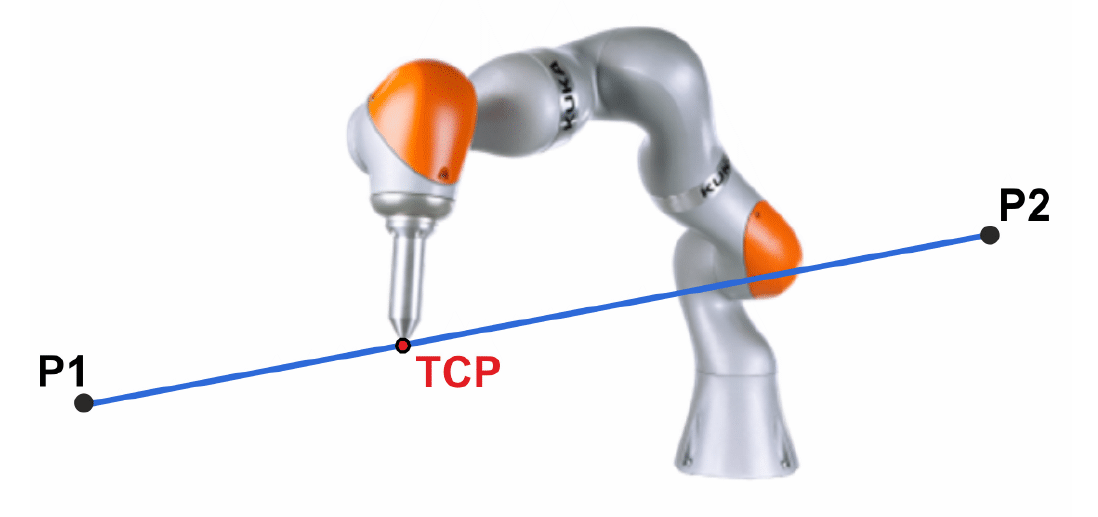
\includegraphics[scale=0.4]{linmotion}
    \caption{LIN mozgás\cite{sunrisemanual}}
    \label{fig:linmotion}
\end{figure}

\newpage
\subsection{A robotkar mozgatása} \label{sec:motionprogramming}
A projekt során a robotkarral egyszerű mozgásokat kellett végeztetni. Nem volt szükség bonyolultabb görbék és felületek lekövetésére, csak ponttól ponttig mozgásra.

A robot mozgása szekvenciálisan ismétlődik, ennek lépései a következők:
\begin{enumerate}
\setcounter{enumi}{-1} 
	\item a robotkar képfelvételi pozícióba vezérlése (a normál játékmenet közben mindig ebből a pozícióból indul, nem kell ide irányítani)
	\item a sakkprogram által meghatározott lépés kezdőmezője fölé irányítása
	\item csökkentett sebességgel a bábuért lenyúlás, majd a gripper záródása után szintén csökkentett sebességgel visszaemelés
	\item a lépés végpontja fölé vezérlés
	\item redukált sebességgel a bábu lerakása, majd a gripper kinyílása után szintén redukált sebességgel visszaemelkedés a bábu fölé
	\item képkészítési pozícióba való visszatérés
\end{enumerate}

A szakdolgozat keretében megírt program nem keresi meg automatikusan az ideális képkészítési pozíciót (továbbfejlesztési irány), ezt kézzel kell megtennünk. Erre a csuklók direkt vezérlése is alkalmas, de praktikusabb egy tetszőleges koordinátarendszerben XYZ tengelyek mentén mozgatni (például a sakktábla sarkán felvett bázis KR-ben).

Ahhoz hogy a kamera látóterébe az egész kalibrációs tábla beleessen a robotkarnak viszonylag magasra kell nyúlnia. Ezt a 7, illetve a 14 kilós iiwa robotkar mozgástere is megengedi. Kisebb méretű robottal a projekt megvalósításához nagyobb látószögű kamerára vagy több képkészítési pozícióra lenne szükség.

\begin{figure}[h]
    \centering
    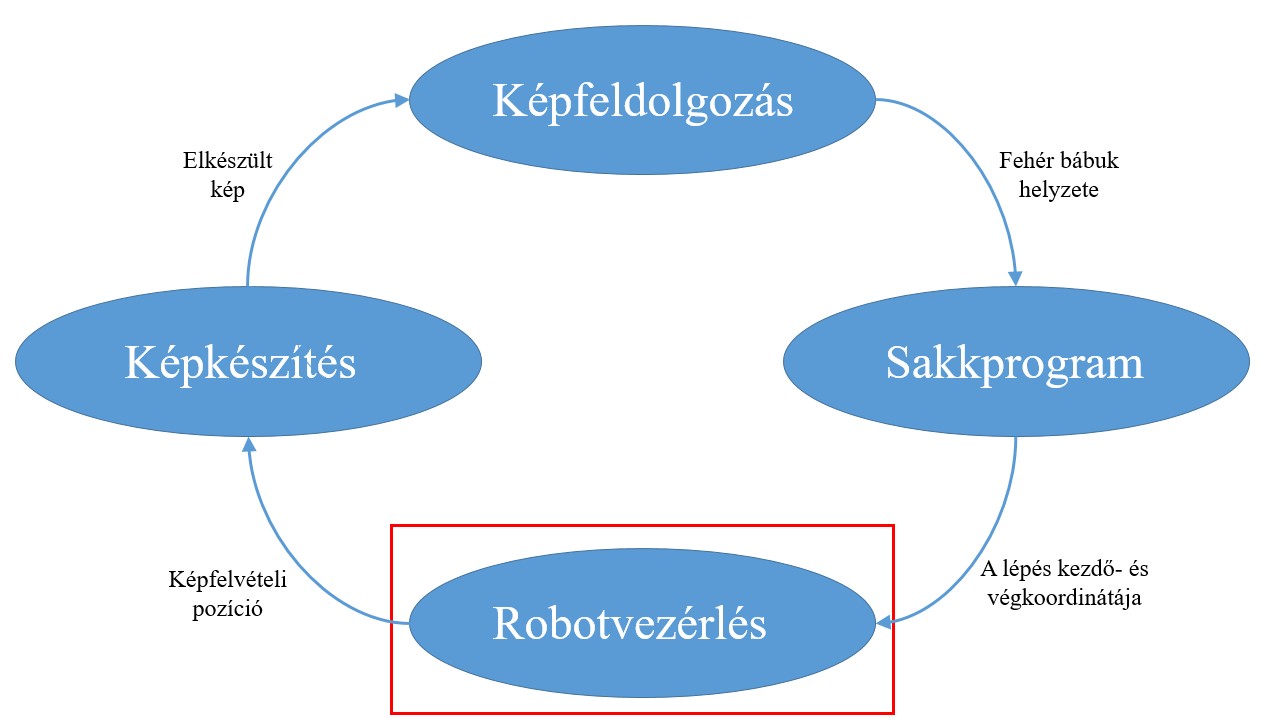
\includegraphics[scale=0.4]{flowchart-robot}
    \caption{A robotvezérlés helye a folyamatban}
    \label{fig:flowchart-robot}
\end{figure}

Praktikus lehet egy olyan frame betanítása, ahol az orientáció olyan, ahogy a robotkarnak a bábut meg kéne fognia. Erről a frame-ről másolatot készítve annak X, Y és Z koordinátáját külön-külön be lehet állítani. A sakktábla bázispont és ez a frame alapján a tábla összes mezőjéhez lehet generálni egy alsó megfogó helyzetet (ahol a megfogó két pofája összezáródik) és egy felsőt, ahová a képkészítés után megy. Az alsó megfogó helyzet a gripper TCP-re vonatkozik, a robotkar mozgatásához célszerű ezt a pontot irányítani.

A hagyományos sakktábla 8x8-as, az alsó és felső pozíciót is beleszámolva ez 128 generált frame-et jelent. Ezek kiszámítása nem különösebben időigényes, de áttekinthetőbb a programkód, ha ezekből a fizikai pozíciókból a sakkprogramhoz hasonlóan egy (az alsó és felső helyzet miatt 2) 8x8-as tömböt építünk fel a sakkprogramhoz hasonló indexeléssel. Mivel a sakktábla méretei ismertek, ezt 2 egymásba ágyazott for ciklussal meg lehet oldani, a bázis koordinátarendszerhez a megfelelő offszetet hozzáadva.

A projekt során a megfogópofa egyik sarokpontja lett betanítva TCP-nek, így szükség van még egy plusz offszetre ahhoz, hogy a robotkar mozgatásakor a megfogó középvonala kerüljön a mező közepe fölé, ne pedig a TCP (\ref{fig:tcp-examples} ábra).

A bábuk mozgatására érdemes külön függvényt írni, ami fogadja a sakkprogram által visszaadott kezdő- és végpont indexeket, majd ez alapján az adott bábut áthelyezi a megfelelő mezőre. A főprogramban implementált `MovePiece' függvény ezt a célt szolgálja. A bábuk emelésekor és letételekor érdemes a PTP mozgatás helyett a LIN-t alkalmazni, mivel annak tetszőlegesen állítható a sebessége\footnote{A PTP esetén is meg lehet adni egy százalékos sebességredukciót a tengelyekre.}.










\end{document}